\documentclass{beamer}
\usetheme{Madrid}
\usepackage[utf8]{inputenc}
\usepackage[T1]{fontenc}
\usepackage{graphicx}
\usepackage{lmodern}
\usepackage{tikz}

% Pour enlever le \institute du bas de page
% Rapetisser les noms et date etc dans le footer
\setbeamertemplate{footline}
{
      \leavevmode%
      \hbox{%
      \begin{beamercolorbox}[wd=.333333\paperwidth,ht=2.25ex,dp=1ex,center]{author in head/foot}%
      \
      \end{beamercolorbox}%
      \begin{beamercolorbox}[wd=.333333\paperwidth,ht=2.25ex,dp=1ex,center]{title in head/foot}%
      \usebeamerfont{title in head/foot}\insertshorttitle
      \end{beamercolorbox}%
      \begin{beamercolorbox}[wd=.333333\paperwidth,ht=2.25ex,dp=1ex,right]{date in head/foot}%
      \usebeamerfont{date in head/foot}\insertshortdate{}\hspace*{2em}
      \insertframenumber{} / \inserttotalframenumber\hspace*{2ex} 
      \end{beamercolorbox}}%
      \vskip0pt%
}

\AtBeginSection[]
{
      \begin{frame}
            \tableofcontents[currentsection,hideallsubsections]
      \end{frame}
}

\title{Tableau virtuel interactif}
\author{\textcolor{blue}{Baptiste Saleil}, \textcolor{cyan}{Geoffrey Mélia}, \textcolor{blue}{Julien Pagès}, \textcolor{cyan}{Kevin Bollini} \\ \ \\Tuteur de projet: M. Puech}
\date{30 avril 2012}

\begin{document}
	%Kevin
	\begin{frame}
		\titlepage
	\end{frame}

	\section{Introduction}
		\begin{frame}{Introduction}
		
		But du projet :
            \begin{itemize}
			\item Proposer un sujet en lien avec nos deux formations
            \item Concevoir une application utilisant les mouvements de l'utilisateur (sans souris)
            \item Développer une bibliothèque de détection d'objet dans une image
            \item Exploiter cette bibliothèque pour reconnaitre les mouvements de l'utilisateur
            \item Pouvoir écrire ou dessiner à plusieurs sur un tableau virtuel
            \end{itemize}
            
            \end{frame}

      \begin{frame}{Vidéo de présentation}
            %\movie{\includegraphics[width=.65\textwidth]{demo}}{demo.ogv}
      \end{frame}

%Plan
      \begin{frame}{Plan}
            \tableofcontents
      \end{frame}
            
      \section{Analyse et Conception}
      \subsection{Choix de conceptions}
            \begin{frame}{Choix de conceptions}
                  \begin{block}{Choix principaux}
                        Découper le projet en deux parties distinctes : \\
                        - une bibliothèque de suivi d'objets réutilisable \\
                        - une application avec une interface naturelle exploitant cette bibliothèque \\
                  \end{block}
            \end{frame}
            
      \subsection{Gestion de projet}
            \begin{frame}{Gestion de projet}
                  \begin{block}{Méthodologie :}
                  \begin{itemize}
                  \item Se renseigner, réaliser une architecture de qualité
                  \item Répartir le travail en fonction des compétences et formations de chacun
                  \item Développer rapidement un prototype
                  \item Développement incrémental en ajoutant des fonctionnalités
                  \end{itemize}
                  \end{block}
            \end{frame}
            
            \begin{frame}{Gestion de projet}
                  \begin{block}{Organisation :}
                  \begin{itemize}
                        \item{Réunions}
                        \item{Deux sous-groupes}
                        \item{Partage des tâches au sein des groupes}
                        \item{Décisions communes (à quatre)}
                  \end{itemize}
                  \end{block}
            
            \begin{block}{Collaboration :}
                  \begin{itemize}
                        \item{Gestionnaire de versions (Subversion)}
                        \item{Partage de documents (Mail et Subversion)}
                        \item{Discussions (Mails / Instantanées)}
                        \item{Édition collaborative pour le travail à distance (Gobby)}
                  \end{itemize}
         \end{block}
            \end{frame}
            
      % Partie de Geoffrey
      \subsection{Analyse}
            \begin{frame}{Analyse}
                  \begin{exampleblock}{Objectifs}
                        \begin{itemize}
                              \item{Identifier les besoins et envies des utilisateurs}
                              \item{Distinguer et classer les fonctionnalités de l'application}
                              \item{Établir un schéma de conception dans le temps}
                              \item{Faciliter le développement, avoir des buts concrets}
                              \item{Produire une application réellement aboutie}
                        \end{itemize}
                  \end{exampleblock}
            \end{frame}
      
      \subsection{Planning}
            \begin{frame}{Rétroplanning}      
                  Rétroplanning (Diagramme de gantt) :
                  \begin{center}
                  % TODO : mettre à jour le rétroplanning
                  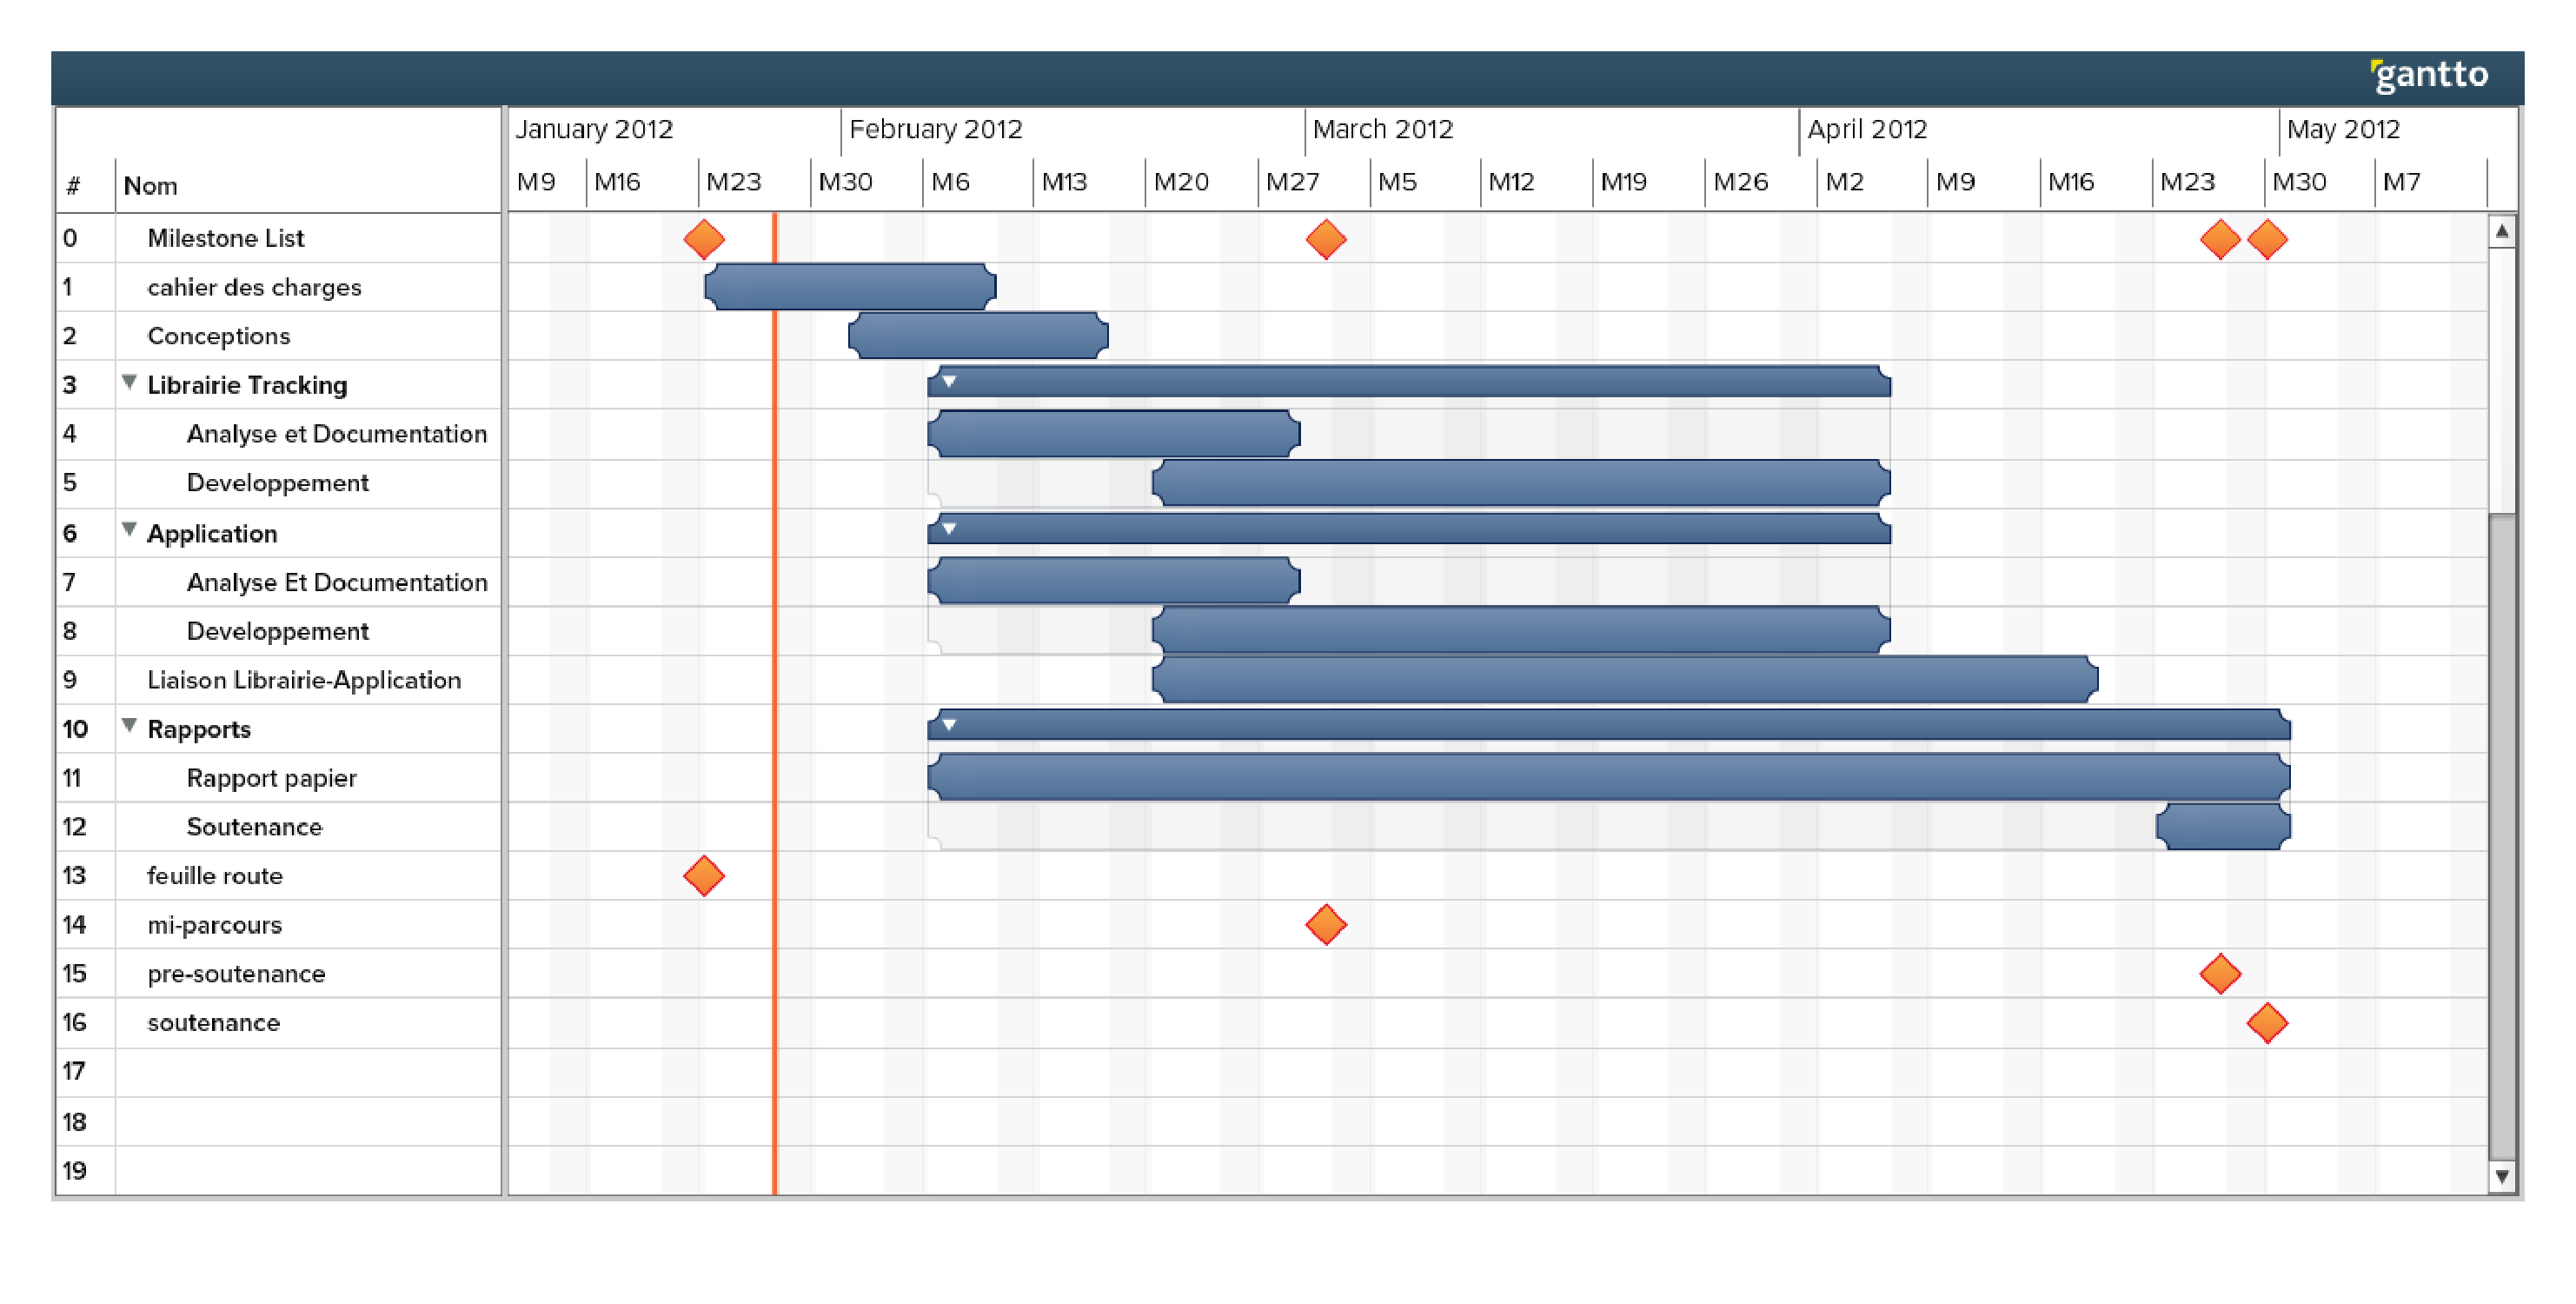
\includegraphics[scale=0.25]{../feuille-route/retroplanning.pdf}
                  \end{center}
            \end{frame}

      %Partie de Kevin Et Geoffrey
      %Geoffrey
      \section{Bibliothèque}
            \subsection{Architecture}
            \begin{frame}{Bibliothèque de suivi d'objets : libtrack}
                  \begin{block}{Objectifs de la bibliothèque conçue}
                        \begin{itemize}
                        \item{Distinguer complètement le suivi d'objet de l'application}
                        \item{Avoir une utilisation simple sans connaissance en traitement d'image}
                        \item{Permettre la détection d'actions}
                        \item{Proposer un maximum de solutions de suivi}
                        \item{Évaluer et comparer ces solutions}
                        \end{itemize}
                  \end{block}
            \end{frame}

            \begin{frame}{Bibliothèque libtrack}
                  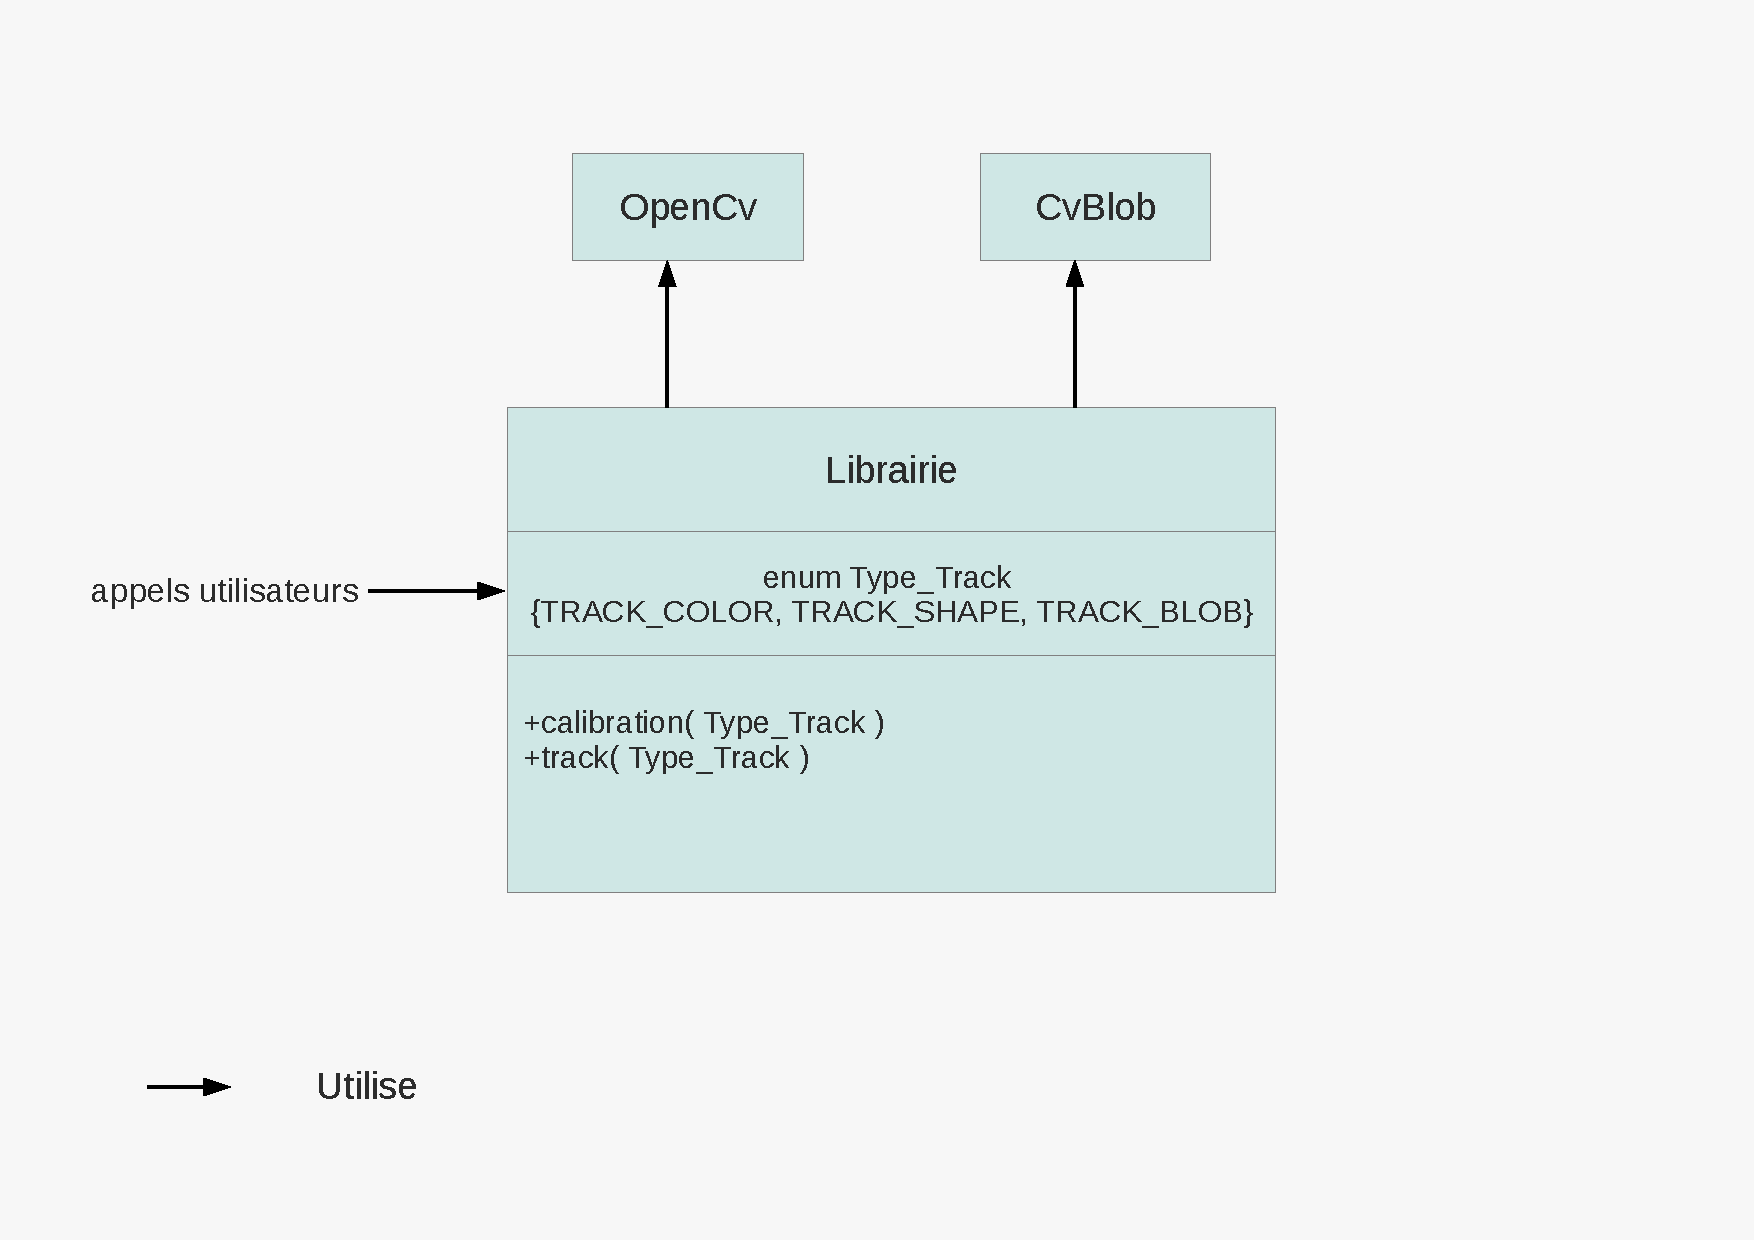
\includegraphics[scale=0.40]{schema-librairie.pdf}
            \end{frame}

            \begin{frame}{Bibliothèque}

            Création d'une structure de données : Cursor\\
    inclure graphique de la structure + énum
            \end{frame}
            
      %TODO frame a supprimer
            \begin{frame}{Bibliothèque}
            Deux fonctions enveloppes : \\
                  \begin{itemize}
                        \item{Cursor * calibration(IplImage * source, CvPoint A, CvPoint B, TYPE-TRACK flag)}
                        \item{int track(IplImage * source, Cursor * oldCursor)}
                  \end{itemize}            
            \end{frame}

            \subsection{Comparatifs des méthodes de suivi}
            \begin{frame}{Comparatif Couleur/modèle}
            \pause
                  \begin{block}{Couleur}
                        Avantages \\
                        - Suivi rapide \\
                        - Diversité possible de curseurs \\
                        Faiblesses \\
                        - Sensibilité à l'environnement\\
                        - Dépendant de la qualité du dispositif d'acquisition\\
                  \end{block}
                  \pause
                  \begin{block}{modèle}
                        Avantages \\
                        - Suivi moins dépendant de la qualité de l'environnement \\
                        - Efficace sur des objets 'complexes'\\
                        Faiblesses \\
                        - Suivi lent \\
                        - Très sensible aux variations du curseur\\
                  \end{block}
            \end{frame}
            \begin{frame}{Comparatif Simple/composante connexe}
            \pause
                  \begin{block}{Barycentre simple}
                        Avantages \\
                        - Suivi rapide \\
                        Faiblesses \\
                        - Sensibilité aux parasites (fausses détections)\\
                        - Précision fortement dépendante de l'environnement\\
                  \end{block}
                  \pause
                  \begin{block}{Barycentre composante connexe}
                        Avantages \\
                        - Suivi plus précis \\
                        - Résistance aux parasites \\
                        Faiblesses \\
                        - Suivi plus lent \\
                        - Perte occasionnelle du curseur
                  \end{block}
            \end{frame}

            %Kevin
            \subsection{Fonctionnement}
            \begin{frame}{Scénario type d'utilisation de la bibliothèque}
                  La bibliothèque s'utilise en deux grandes étapes :
                  \begin{itemize}
                        \item{Calibration, engendrant une struture Cursor}
                        \item{Track, mettant à jour les informations de la structure}
                  \end{itemize}
            \end{frame}

            \subsubsection{Calibration}
            \begin{frame}{Calibration : Source d'images et TYPE\_TRACK}
                  \begin{center}
                        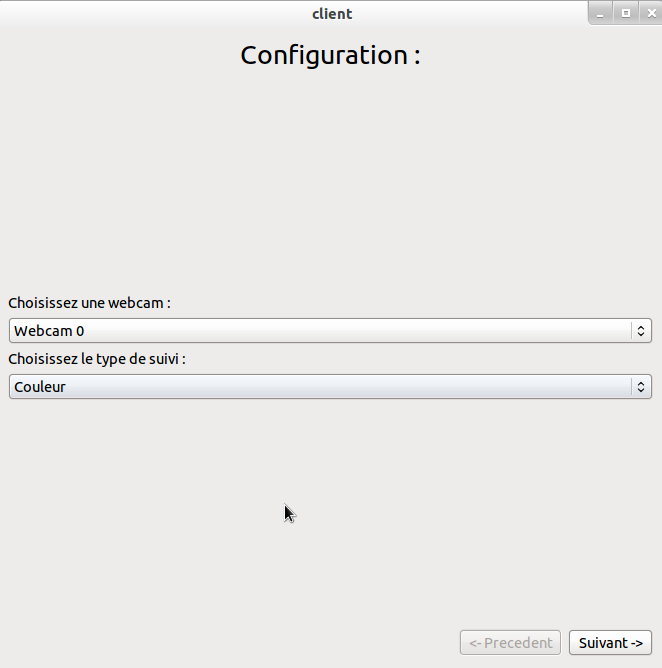
\includegraphics[scale=0.25]{Capture6.png}\\
                        Écran de sélection du Type\_TRACK et de la source d'images
                  \end{center}
            \end{frame}

            \begin{frame}{Calibration : Sélection du curseur}
                  \begin{itemize}
                        \item{Extrait la position de l'objet à suivre}
                  \end{itemize}
                  \begin{center}
                        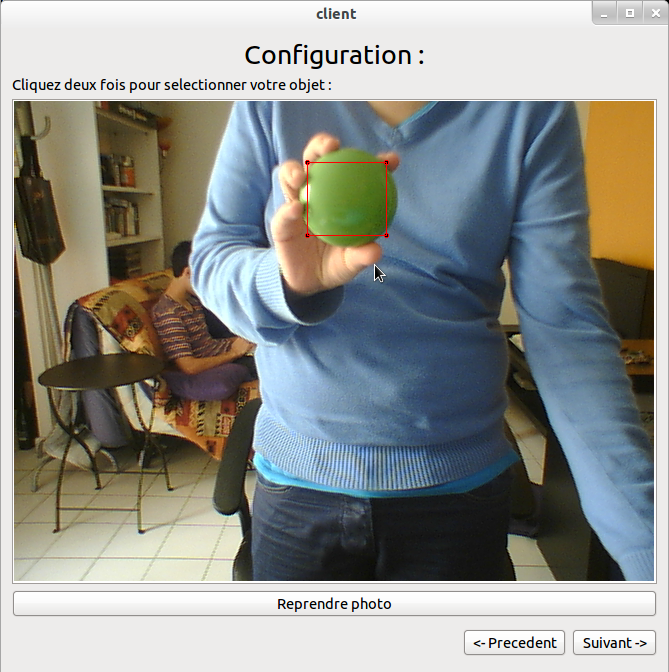
\includegraphics[scale=0.25]{Capture1.png}\\
                        Sélection de l'objet
                  \end{center}
            
            \end{frame}

            \begin{frame}{Calibration couleur : Réglage du seuil}
                  \begin{itemize}
                        \item{Modifie l'attribut "threshold" de la structure Cursor.}
                  \end{itemize}
                  \begin{center}
                        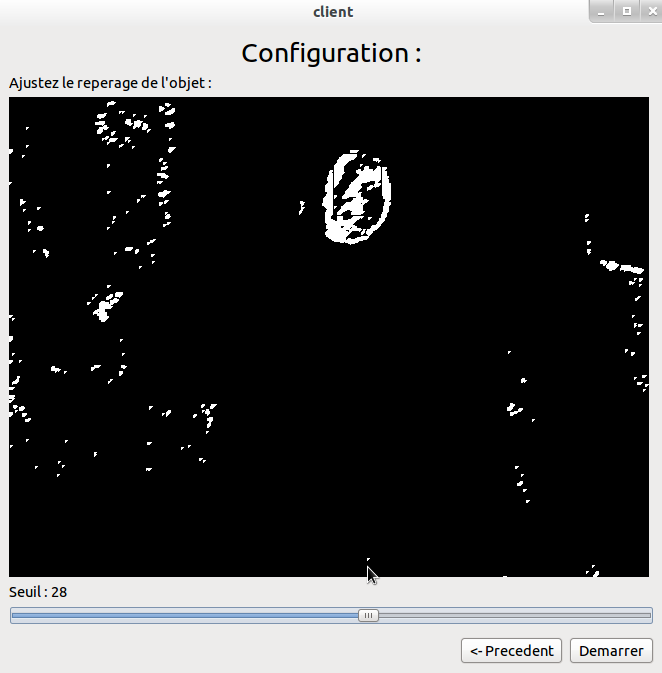
\includegraphics[scale=0.25]{Capture2.png}\\
                        Écran de réglage du seuil
                  \end{center}
            \end{frame}
            
            \subsubsection{Suivi}
            \begin{frame}{Suivi par couleur : Barycentre}
                  \begin{center}
                        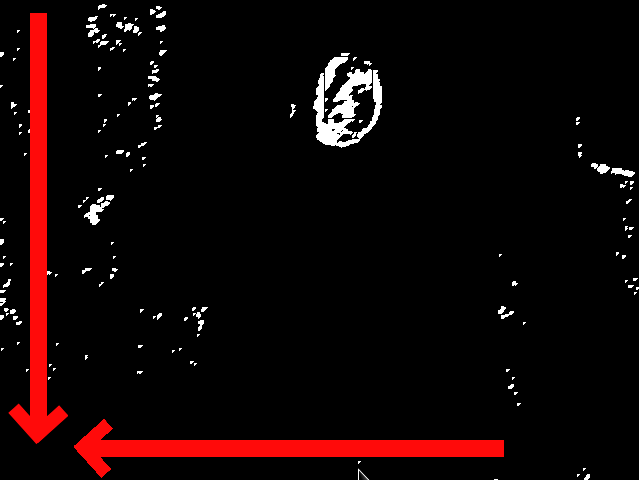
\includegraphics[scale=0.25]{Capture4.png}\\
                        Calcul du barycentre de l'image binaire
                  \end{center}
            \end{frame}

            \begin{frame}{Suivi par Blob : Composantes connexes}
                  \begin{center}
                        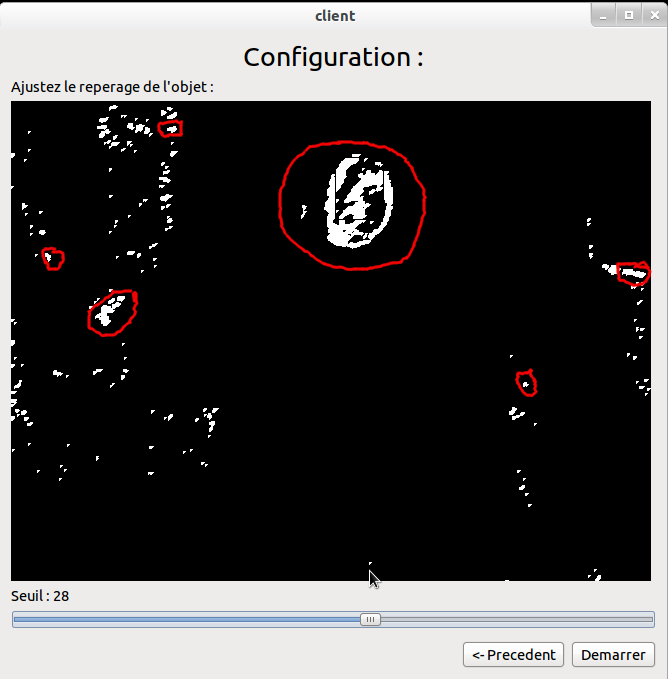
\includegraphics[scale=0.25]{Capture5.png}\\
                        Recherche et isolement de la composante connexe pertinante
                  \end{center}
            \end{frame}

            \begin{frame}{Suivi par couleur/Blob : Détection d'action}
                  \begin{itemize}
                        \item{Détection d'action par approchement du curseur}
                  \end{itemize}
                  \begin{center}
                        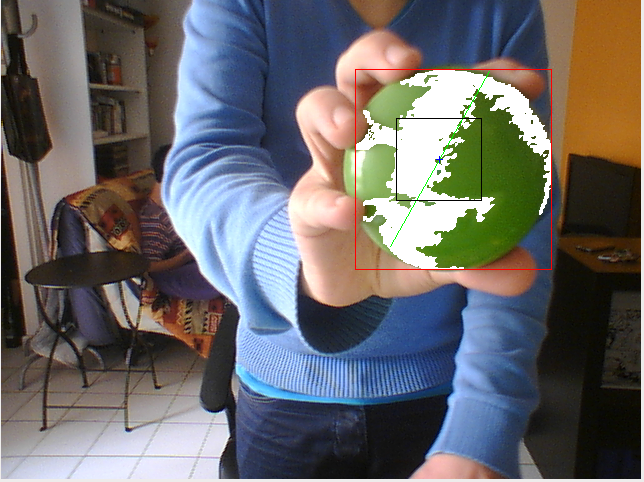
\includegraphics[scale=0.25]{Capture3.png}\\
                        Retour image de l'objet suivi
                  \end{center}
            \end{frame}
            %Kevin
            \begin{frame}{Suivi par modèle}
                  \begin{itemize}
                        \item{Recherche du template dans l'image}
                  \end{itemize}
            \end{frame}
            

            \begin{frame}{Bilan}
                  \begin{exampleblock}{Objectifs atteints}
                        \begin{itemize}
                        \item Bibliothèque utilisable et proposant plusieurs solutions de suivi
                        \item Détection d'action implémentée dans deux des trois solutions
                        \item Utilisation simple sans connaissances en traitement d'images
                        \end{itemize}
                  \end{exampleblock}
                  \pause
                  \begin{alertblock}{Difficultés et ouverture}
                        \begin{itemize}
                        \item Temps d'adaptation aux bibliothèques OpenCv et CvBlob volumineux
                        \item Implémentation de la détection pour le suivi par modèle
                        \item Ajout à la bibliothèque de nouvelles fonctions de suivi
                        \end{itemize}
                  \end{alertblock}
				  
                  \begin{block}{Ouverture}
                        - Diversifier et optimiser les méthodes de suivi \\
                        - Rajouter des fonctionnalités côté application \\
                  \end{block}				  
            \end{frame}
      
 	% Baptiste et Julien
	% Baptiste
	
	\section{Application}
	
		\subsection{Objectifs}
		\begin{frame}{Objectifs}
			\begin{itemize}
				\item Interface intuitive
				\item Modulable, Extensible
				\item Fonctionnement transparent mode local / mode réseau
				\item Séparer le traitement du rendu
				\item Etablir un protocole simple et rapide
			\end{itemize}
		\end{frame}
	
		\subsection{Architecture}
		\begin{frame}{Architecture - Modules}
			\pause
			\begin{block}{Etalonnage}
				\begin{itemize}
					\item Choix principaux
					\item Réglages
				\end{itemize}
			\end{block}
			\pause
			\begin{block}{Client}
				\begin{itemize}
					\item Interface graphique
					\item Liens entre les modules
				\end{itemize}
			\end{block}
			\pause
			\begin{block}{Tableau}
				\begin{itemize}
					\item Dessin / Interface gestuelle
					\item Réseau
				\end{itemize}
			\end{block}
			\pause
			\begin{block}{Serveur}
				\begin{itemize}
					\item Communication entre clients
					\item Synchronisatoin du tableau
				\end{itemize}
			\end{block}
		\end{frame}
	
		\begin{frame}{Architecture - Classes}
			\begin{center}		
				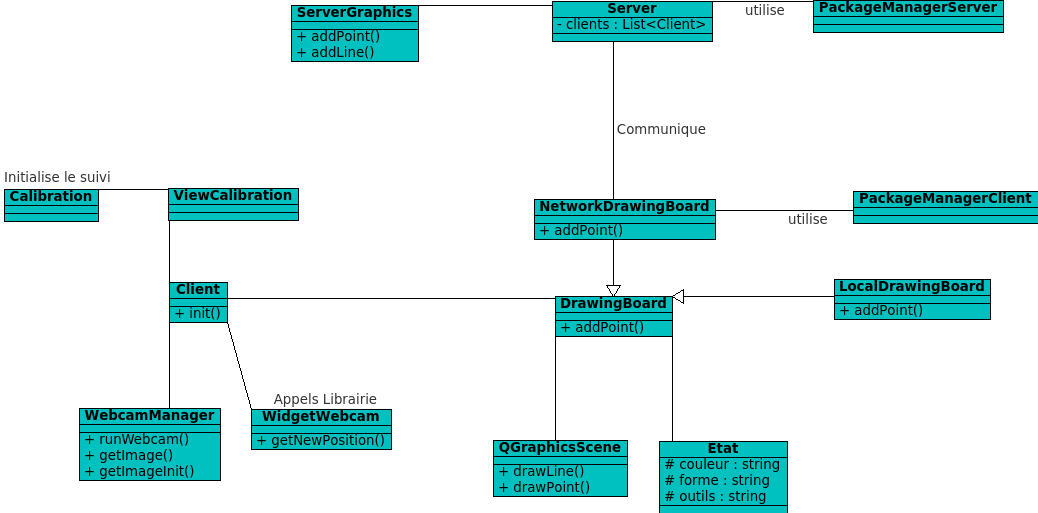
\includegraphics[scale=0.45]{../uml/classes.png}
			\end{center}
		\end{frame}
		
		\subsection{Fonctionnalités}
		\begin{frame}{Fonctionnalités - Outils}
			\begin{center}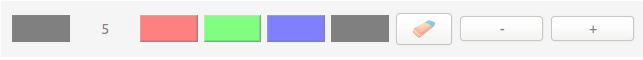
\includegraphics[scale=0.45]{toolbar.png}\end{center}
			\begin{center}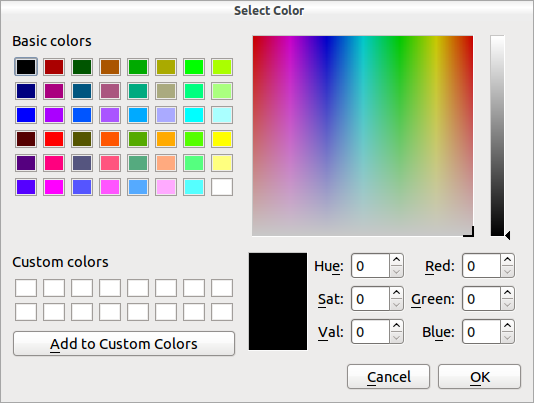
\includegraphics[scale=0.2]{colorpicker.png}\end{center}
			\begin{itemize}
				\item Couleur
				\item Gomme
				\item Taille
				\item Affichage
			\end{itemize}
		\end{frame}
		\begin{frame}{Fonctionnalités - Actions}
			\begin{center}
				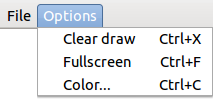
\includegraphics[scale=0.6]{menu.png}\quad
				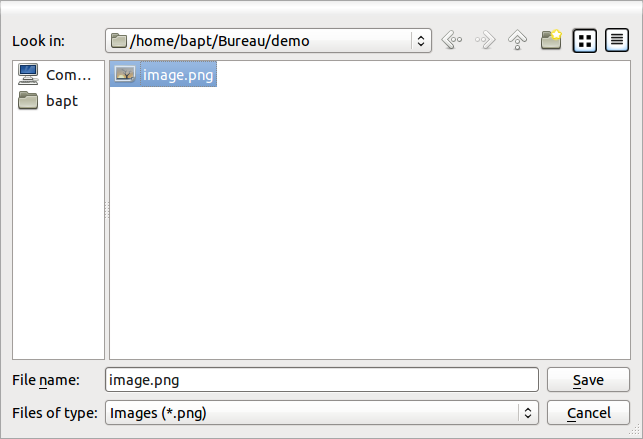
\includegraphics[scale=0.2]{export.png}
			\end{center}
			\begin{itemize}
				\item Sauvegarde
				\item Vider le dessin
				\item Mode plein écran
			\end{itemize}
		\end{frame}
		
		\subsection{Fonctionnement}
		\begin{frame}{Fonctionnement - Interface intuitive}
			\begin{center}
				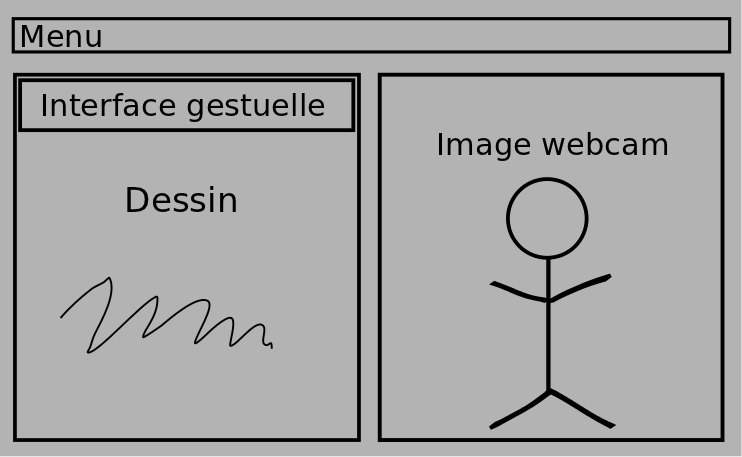
\includegraphics[scale=0.45]{interface.png}
			\end{center}
		\end{frame}
		
		\begin{frame}{Fonctionnement - Etalonnage}
			\begin{block}{Technique}
				\begin{itemize}
					\item Interface "Suivant - Précédent"
					\item Etalonnage obligatoire
				\end{itemize}
			\end{block}
			\begin{block}{Utilisation}
				\begin{enumerate}
					\item Choix webcam / Type de suivi
					\item Sélection de l'objet
					\item Réglage de la détection
					\item Choix mode local / réseau
				\end{enumerate}
			\end{block}
			
		\end{frame}
		
		\begin{frame}{Fonctionnement - Local}
			Pseudo-séquence + explications
		\end{frame}
		
		\begin{frame}{Fonctionnement - Réseau}
			Pseudo-séquence + explications
		\end{frame}
		
		\subsection{Mise en production}
		\begin{frame}{Mise en production}
			\begin{block}{Pourquoi?}
				\begin{itemize}
					\item Généralement oubliée
					\item Première expérience
					\item Application aboutie
				\end{itemize}
			\end{block}
			\begin{block}{Eléments}
				\begin{itemize}
					\item Traduction
					\item Packaging
					\item Documentation
					\item Portabilité
					\item Dépôt accessible
					\item Code propre
				\end{itemize}
			\end{block}
		\end{frame}
		
		\subsection{Ouverture}
		\begin{frame}{Ouverture}
			\begin{itemize}
				\item Amélioration du réseau
				\item Amélioration des performances
				\item Possibilité de relancer l'étalonnage
			\end{itemize}
		\end{frame}
		
		% \scalebox{0.5}{% Graphic for TeX using PGF
% Title: /home/julien/master/projet/dessin-realite-augmentee/documents/uml/sequence_reseau.dia
% Creator: Dia v0.97.2
% CreationDate: Tue Apr 24 10:47:45 2012
% For: julien
% \usepackage{tikz}
% The following commands are not supported in PSTricks at present
% We define them conditionally, so when they are implemented,
% this pgf file will use them.
\ifx\du\undefined
  \newlength{\du}
\fi
\setlength{\du}{15\unitlength}
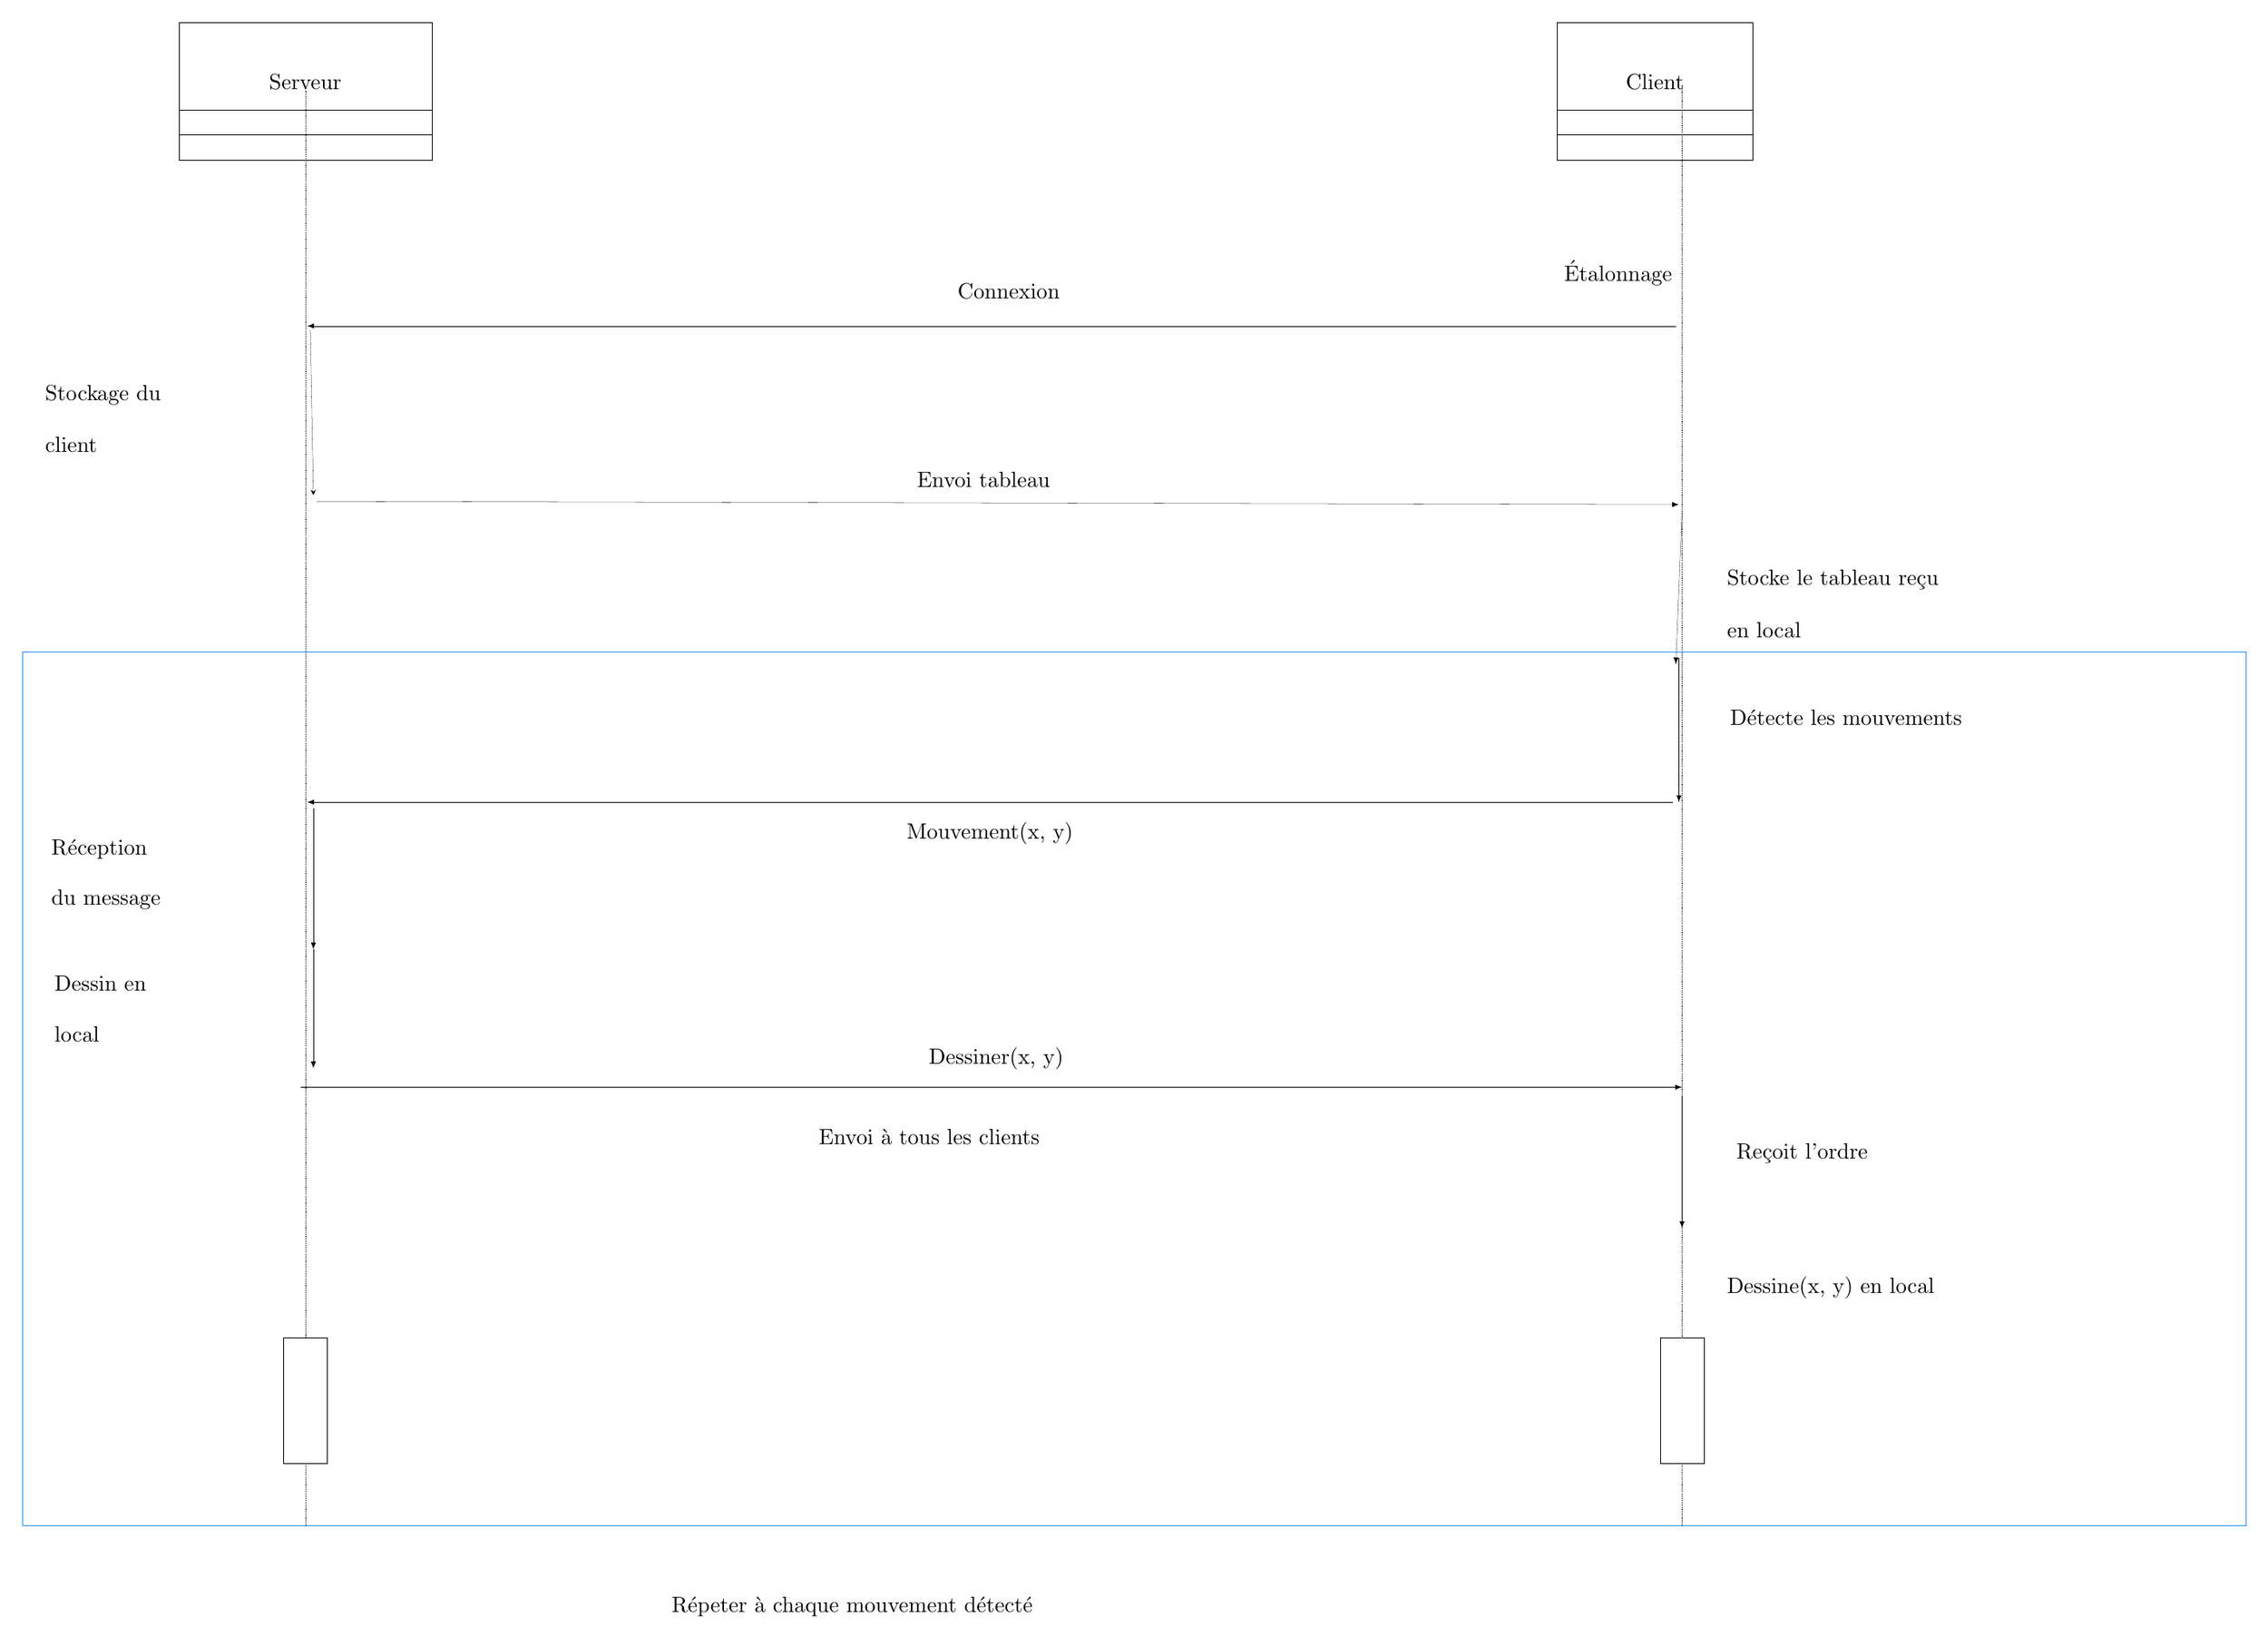
\begin{tikzpicture}
\pgftransformxscale{1.000000}
\pgftransformyscale{-1.000000}
\definecolor{dialinecolor}{rgb}{0.000000, 0.000000, 0.000000}
\pgfsetstrokecolor{dialinecolor}
\definecolor{dialinecolor}{rgb}{1.000000, 1.000000, 1.000000}
\pgfsetfillcolor{dialinecolor}
\pgfsetlinewidth{0.100000\du}
\pgfsetdash{}{0pt}
\definecolor{dialinecolor}{rgb}{1.000000, 1.000000, 1.000000}
\pgfsetfillcolor{dialinecolor}
\fill (5.000000\du,7.000000\du)--(5.000000\du,8.400000\du)--(9.042500\du,8.400000\du)--(9.042500\du,7.000000\du)--cycle;
\definecolor{dialinecolor}{rgb}{0.000000, 0.000000, 0.000000}
\pgfsetstrokecolor{dialinecolor}
\draw (5.000000\du,7.000000\du)--(5.000000\du,8.400000\du)--(9.042500\du,8.400000\du)--(9.042500\du,7.000000\du)--cycle;
% setfont left to latex
\definecolor{dialinecolor}{rgb}{0.000000, 0.000000, 0.000000}
\pgfsetstrokecolor{dialinecolor}
\node at (7.021250\du,7.950000\du){Serveur};
\definecolor{dialinecolor}{rgb}{1.000000, 1.000000, 1.000000}
\pgfsetfillcolor{dialinecolor}
\fill (5.000000\du,8.400000\du)--(5.000000\du,8.800000\du)--(9.042500\du,8.800000\du)--(9.042500\du,8.400000\du)--cycle;
\definecolor{dialinecolor}{rgb}{0.000000, 0.000000, 0.000000}
\pgfsetstrokecolor{dialinecolor}
\draw (5.000000\du,8.400000\du)--(5.000000\du,8.800000\du)--(9.042500\du,8.800000\du)--(9.042500\du,8.400000\du)--cycle;
\definecolor{dialinecolor}{rgb}{1.000000, 1.000000, 1.000000}
\pgfsetfillcolor{dialinecolor}
\fill (5.000000\du,8.800000\du)--(5.000000\du,9.200000\du)--(9.042500\du,9.200000\du)--(9.042500\du,8.800000\du)--cycle;
\definecolor{dialinecolor}{rgb}{0.000000, 0.000000, 0.000000}
\pgfsetstrokecolor{dialinecolor}
\draw (5.000000\du,8.800000\du)--(5.000000\du,9.200000\du)--(9.042500\du,9.200000\du)--(9.042500\du,8.800000\du)--cycle;
\pgfsetlinewidth{0.100000\du}
\pgfsetdash{}{0pt}
\definecolor{dialinecolor}{rgb}{1.000000, 1.000000, 1.000000}
\pgfsetfillcolor{dialinecolor}
\fill (27.000000\du,7.000000\du)--(27.000000\du,8.400000\du)--(30.132500\du,8.400000\du)--(30.132500\du,7.000000\du)--cycle;
\definecolor{dialinecolor}{rgb}{0.000000, 0.000000, 0.000000}
\pgfsetstrokecolor{dialinecolor}
\draw (27.000000\du,7.000000\du)--(27.000000\du,8.400000\du)--(30.132500\du,8.400000\du)--(30.132500\du,7.000000\du)--cycle;
% setfont left to latex
\definecolor{dialinecolor}{rgb}{0.000000, 0.000000, 0.000000}
\pgfsetstrokecolor{dialinecolor}
\node at (28.566250\du,7.950000\du){Client};
\definecolor{dialinecolor}{rgb}{1.000000, 1.000000, 1.000000}
\pgfsetfillcolor{dialinecolor}
\fill (27.000000\du,8.400000\du)--(27.000000\du,8.800000\du)--(30.132500\du,8.800000\du)--(30.132500\du,8.400000\du)--cycle;
\definecolor{dialinecolor}{rgb}{0.000000, 0.000000, 0.000000}
\pgfsetstrokecolor{dialinecolor}
\draw (27.000000\du,8.400000\du)--(27.000000\du,8.800000\du)--(30.132500\du,8.800000\du)--(30.132500\du,8.400000\du)--cycle;
\definecolor{dialinecolor}{rgb}{1.000000, 1.000000, 1.000000}
\pgfsetfillcolor{dialinecolor}
\fill (27.000000\du,8.800000\du)--(27.000000\du,9.200000\du)--(30.132500\du,9.200000\du)--(30.132500\du,8.800000\du)--cycle;
\definecolor{dialinecolor}{rgb}{0.000000, 0.000000, 0.000000}
\pgfsetstrokecolor{dialinecolor}
\draw (27.000000\du,8.800000\du)--(27.000000\du,9.200000\du)--(30.132500\du,9.200000\du)--(30.132500\du,8.800000\du)--cycle;
\pgfsetlinewidth{0.050000\du}
\pgfsetdash{}{0pt}
\pgfsetdash{{0.400000\du}{0.400000\du}}{0\du}
\definecolor{dialinecolor}{rgb}{0.000000, 0.000000, 0.000000}
\pgfsetstrokecolor{dialinecolor}
\draw (29.000000\du,8.000000\du)--(29.000000\du,28.000000\du);
\definecolor{dialinecolor}{rgb}{0.000000, 0.000000, 0.000000}
\pgfsetstrokecolor{dialinecolor}
\draw (29.000000\du,30.000000\du)--(29.000000\du,31.000000\du);
\pgfsetlinewidth{0.100000\du}
\pgfsetdash{}{0pt}
\definecolor{dialinecolor}{rgb}{1.000000, 1.000000, 1.000000}
\pgfsetfillcolor{dialinecolor}
\fill (28.650000\du,28.000000\du)--(28.650000\du,30.000000\du)--(29.350000\du,30.000000\du)--(29.350000\du,28.000000\du)--cycle;
\definecolor{dialinecolor}{rgb}{0.000000, 0.000000, 0.000000}
\pgfsetstrokecolor{dialinecolor}
\draw (28.650000\du,28.000000\du)--(28.650000\du,30.000000\du)--(29.350000\du,30.000000\du)--(29.350000\du,28.000000\du)--cycle;
\pgfsetlinewidth{0.050000\du}
\pgfsetdash{}{0pt}
\pgfsetdash{{0.400000\du}{0.400000\du}}{0\du}
\definecolor{dialinecolor}{rgb}{0.000000, 0.000000, 0.000000}
\pgfsetstrokecolor{dialinecolor}
\draw (7.021250\du,8.100000\du)--(7.021250\du,28.000000\du);
\definecolor{dialinecolor}{rgb}{0.000000, 0.000000, 0.000000}
\pgfsetstrokecolor{dialinecolor}
\draw (7.021250\du,30.000000\du)--(7.021250\du,31.000000\du);
\pgfsetlinewidth{0.100000\du}
\pgfsetdash{}{0pt}
\definecolor{dialinecolor}{rgb}{1.000000, 1.000000, 1.000000}
\pgfsetfillcolor{dialinecolor}
\fill (6.671250\du,28.000000\du)--(6.671250\du,30.000000\du)--(7.371250\du,30.000000\du)--(7.371250\du,28.000000\du)--cycle;
\definecolor{dialinecolor}{rgb}{0.000000, 0.000000, 0.000000}
\pgfsetstrokecolor{dialinecolor}
\draw (6.671250\du,28.000000\du)--(6.671250\du,30.000000\du)--(7.371250\du,30.000000\du)--(7.371250\du,28.000000\du)--cycle;
\pgfsetlinewidth{0.100000\du}
\pgfsetbuttcap
\pgfsetdash{}{0pt}
{
\definecolor{dialinecolor}{rgb}{0.000000, 0.000000, 0.000000}
\pgfsetfillcolor{dialinecolor}
% was here!!!
\pgfsetarrowsstart{latex}
\definecolor{dialinecolor}{rgb}{0.000000, 0.000000, 0.000000}
\pgfsetstrokecolor{dialinecolor}
\draw (7.050000\du,11.850000\du)--(28.900000\du,11.850000\du);
}
% setfont left to latex
\definecolor{dialinecolor}{rgb}{0.000000, 0.000000, 0.000000}
\pgfsetstrokecolor{dialinecolor}
\node at (18.250000\du,11.300000\du){Connexion};
\pgfsetlinewidth{0.100000\du}
\pgfsetdash{}{0pt}
\pgfsetdash{}{0pt}
\pgfsetbuttcap
{
\definecolor{dialinecolor}{rgb}{0.000000, 0.000000, 0.000000}
\pgfsetfillcolor{dialinecolor}
% was here!!!
\pgfsetarrowsend{stealth}
\definecolor{dialinecolor}{rgb}{0.000000, 0.000000, 0.000000}
\pgfsetstrokecolor{dialinecolor}
\draw (7.100000\du,11.900000\du)--(7.150000\du,14.550000\du);
}
\pgfsetlinewidth{0.100000\du}
\pgfsetbuttcap
\pgfsetdash{}{0pt}
{
\definecolor{dialinecolor}{rgb}{0.000000, 0.000000, 0.000000}
\pgfsetfillcolor{dialinecolor}
% was here!!!
\pgfsetarrowsstart{latex}
\definecolor{dialinecolor}{rgb}{0.000000, 0.000000, 0.000000}
\pgfsetstrokecolor{dialinecolor}
\draw (28.950000\du,14.700000\du)--(7.200000\du,14.650000\du);
}
% setfont left to latex
\definecolor{dialinecolor}{rgb}{0.000000, 0.000000, 0.000000}
\pgfsetstrokecolor{dialinecolor}
\node at (17.850000\du,14.300000\du){Envoi tableau};
% setfont left to latex
\definecolor{dialinecolor}{rgb}{0.000000, 0.000000, 0.000000}
\pgfsetstrokecolor{dialinecolor}
\node[anchor=west] at (27.000000\du,11.000000\du){Étalonnage};
% setfont left to latex
\definecolor{dialinecolor}{rgb}{0.000000, 0.000000, 0.000000}
\pgfsetstrokecolor{dialinecolor}
\node[anchor=west] at (2.750000\du,12.950000\du){Stockage du };
% setfont left to latex
\definecolor{dialinecolor}{rgb}{0.000000, 0.000000, 0.000000}
\pgfsetstrokecolor{dialinecolor}
\node[anchor=west] at (2.750000\du,13.750000\du){client};
\pgfsetlinewidth{0.100000\du}
\pgfsetbuttcap
\pgfsetdash{}{0pt}
{
\definecolor{dialinecolor}{rgb}{0.000000, 0.000000, 0.000000}
\pgfsetfillcolor{dialinecolor}
% was here!!!
\pgfsetarrowsstart{latex}
\definecolor{dialinecolor}{rgb}{0.000000, 0.000000, 0.000000}
\pgfsetstrokecolor{dialinecolor}
\draw (28.900000\du,17.250000\du)--(29.000000\du,14.800000\du);
}
% setfont left to latex
% setfont left to latex
\definecolor{dialinecolor}{rgb}{0.000000, 0.000000, 0.000000}
\pgfsetstrokecolor{dialinecolor}
\node[anchor=west] at (29.600000\du,15.900000\du){Stocke le tableau reçu};
% setfont left to latex
\definecolor{dialinecolor}{rgb}{0.000000, 0.000000, 0.000000}
\pgfsetstrokecolor{dialinecolor}
\node[anchor=west] at (29.600000\du,16.700000\du){en local};
\pgfsetlinewidth{0.100000\du}
\pgfsetbuttcap
\pgfsetdash{}{0pt}
{
\definecolor{dialinecolor}{rgb}{0.000000, 0.000000, 0.000000}
\pgfsetfillcolor{dialinecolor}
% was here!!!
\pgfsetarrowsstart{latex}
\definecolor{dialinecolor}{rgb}{0.000000, 0.000000, 0.000000}
\pgfsetstrokecolor{dialinecolor}
\draw (7.050000\du,19.450000\du)--(28.850000\du,19.450000\du);
}
% setfont left to latex
\definecolor{dialinecolor}{rgb}{0.000000, 0.000000, 0.000000}
\pgfsetstrokecolor{dialinecolor}
\node at (17.950000\du,19.950000\du){Mouvement(x, y)};
% setfont left to latex
\definecolor{dialinecolor}{rgb}{0.000000, 0.000000, 0.000000}
\pgfsetstrokecolor{dialinecolor}
\node[anchor=west] at (2.850000\du,20.200000\du){Réception };
% setfont left to latex
\definecolor{dialinecolor}{rgb}{0.000000, 0.000000, 0.000000}
\pgfsetstrokecolor{dialinecolor}
\node[anchor=west] at (2.850000\du,21.000000\du){du message};
% setfont left to latex
\definecolor{dialinecolor}{rgb}{0.000000, 0.000000, 0.000000}
\pgfsetstrokecolor{dialinecolor}
\node[anchor=west] at (2.900000\du,22.350000\du){Dessin en};
% setfont left to latex
\definecolor{dialinecolor}{rgb}{0.000000, 0.000000, 0.000000}
\pgfsetstrokecolor{dialinecolor}
\node[anchor=west] at (2.900000\du,23.150000\du){local};
\pgfsetlinewidth{0.100000\du}
\pgfsetbuttcap
\pgfsetdash{}{0pt}
{
\definecolor{dialinecolor}{rgb}{0.000000, 0.000000, 0.000000}
\pgfsetfillcolor{dialinecolor}
% was here!!!
\pgfsetarrowsstart{latex}
\definecolor{dialinecolor}{rgb}{0.000000, 0.000000, 0.000000}
\pgfsetstrokecolor{dialinecolor}
\draw (7.150000\du,21.800000\du)--(7.150000\du,19.550000\du);
}
% setfont left to latex
\pgfsetlinewidth{0.100000\du}
\pgfsetbuttcap
\pgfsetdash{}{0pt}
{
\definecolor{dialinecolor}{rgb}{0.000000, 0.000000, 0.000000}
\pgfsetfillcolor{dialinecolor}
% was here!!!
\pgfsetarrowsstart{latex}
\definecolor{dialinecolor}{rgb}{0.000000, 0.000000, 0.000000}
\pgfsetstrokecolor{dialinecolor}
\draw (7.150000\du,23.700000\du)--(7.150000\du,21.800000\du);
}
% setfont left to latex
\pgfsetlinewidth{0.100000\du}
\pgfsetbuttcap
\pgfsetdash{}{0pt}
{
\definecolor{dialinecolor}{rgb}{0.000000, 0.000000, 0.000000}
\pgfsetfillcolor{dialinecolor}
% was here!!!
\pgfsetarrowsstart{latex}
\definecolor{dialinecolor}{rgb}{0.000000, 0.000000, 0.000000}
\pgfsetstrokecolor{dialinecolor}
\draw (28.950000\du,19.450000\du)--(28.950000\du,17.150000\du);
}
% setfont left to latex
% setfont left to latex
\definecolor{dialinecolor}{rgb}{0.000000, 0.000000, 0.000000}
\pgfsetstrokecolor{dialinecolor}
\node[anchor=west] at (29.650000\du,18.100000\du){Détecte les mouvements};
\pgfsetlinewidth{0.100000\du}
\pgfsetbuttcap
\pgfsetdash{}{0pt}
{
\definecolor{dialinecolor}{rgb}{0.000000, 0.000000, 0.000000}
\pgfsetfillcolor{dialinecolor}
% was here!!!
\pgfsetarrowsstart{latex}
\definecolor{dialinecolor}{rgb}{0.000000, 0.000000, 0.000000}
\pgfsetstrokecolor{dialinecolor}
\draw (29.000000\du,24.000000\du)--(6.950000\du,24.000000\du);
}
% setfont left to latex
\definecolor{dialinecolor}{rgb}{0.000000, 0.000000, 0.000000}
\pgfsetstrokecolor{dialinecolor}
\node at (18.050000\du,23.550000\du){Dessiner(x, y)};
% setfont left to latex
\definecolor{dialinecolor}{rgb}{0.000000, 0.000000, 0.000000}
\pgfsetstrokecolor{dialinecolor}
\node[anchor=west] at (15.100000\du,24.800000\du){Envoi à tous les clients};
\pgfsetlinewidth{0.100000\du}
\pgfsetbuttcap
\pgfsetdash{}{0pt}
{
\definecolor{dialinecolor}{rgb}{0.000000, 0.000000, 0.000000}
\pgfsetfillcolor{dialinecolor}
% was here!!!
\pgfsetarrowsstart{latex}
\definecolor{dialinecolor}{rgb}{0.000000, 0.000000, 0.000000}
\pgfsetstrokecolor{dialinecolor}
\draw (29.000000\du,26.250000\du)--(29.000000\du,24.150000\du);
}
% setfont left to latex
% setfont left to latex
\definecolor{dialinecolor}{rgb}{0.000000, 0.000000, 0.000000}
\pgfsetstrokecolor{dialinecolor}
\node[anchor=west] at (29.750000\du,25.050000\du){Reçoit l'ordre};
% setfont left to latex
\definecolor{dialinecolor}{rgb}{0.000000, 0.000000, 0.000000}
\pgfsetstrokecolor{dialinecolor}
\node[anchor=west] at (29.600000\du,27.200000\du){Dessine(x, y) en local};
\pgfsetlinewidth{0.100000\du}
\pgfsetdash{}{0pt}
\pgfsetdash{}{0pt}
\pgfsetmiterjoin
\definecolor{dialinecolor}{rgb}{0.117647, 0.564706, 1.000000}
\pgfsetstrokecolor{dialinecolor}
\draw (2.500000\du,17.050000\du)--(2.500000\du,31.000000\du)--(38.000000\du,31.000000\du)--(38.000000\du,17.050000\du)--cycle;
% setfont left to latex
\definecolor{dialinecolor}{rgb}{0.117647, 0.564706, 1.000000}
\pgfsetstrokecolor{dialinecolor}
\node[anchor=west] at (12.750000\du,32.300000\du){Répeter à chaque mouvement détecté};
\end{tikzpicture}
} 

	
      \section{Conclusion}
            \begin{frame}{Conclusion}
                  \begin{exampleblock}{Objectifs atteints}
					\begin{itemize}
                        \item Solution fonctionnelle \\
                        \item Respect du cahier des charges \\
                        \item Découverte (Technologies, gestion de projet...) \\ 
					\end{itemize}
                  \end{exampleblock}
                  \pause
                  \begin{alertblock}{Difficultés}
					\begin{itemize}
                        \item Collaboration : Développement incrémental qui oblige à beaucoup communiquer \\
                        \item Formation : Traitement de l'image, Conception d'architectures \\
                        \item Techniques : Architecture, Fuites de mémoire...\\
					\end{itemize}
                  \end{alertblock}
                  \pause
                  \begin{block}{Ouverture}
					\begin{itemize}
                        \item Diversifier et optimiser les méthodes de suivi \\
                        \item Rajouter des fonctionnalités côté application \\
					\end{itemize}
                  \end{block}
            \end{frame}
      
      \begin{frame}{Sources et bibliographie}
   %need tiny{}
   \begin{itemize}
	\item{\url{http://www.sciencedirect.com.www.ezp.biu-montpellier.fr/science/article/pii/S026288561100120X}}
	\item{\url{http://www.irit.fr/recherches/SAMOVA/pageAnalysis.html}}
	\item{\url{http://www.irit.fr/~Philippe.Joly/Teaching/L3SI/ti.html}}
	\item{\url{http://opencv.willowgarage.com/wiki/}}
	\item{\url{code.google.com/p/cvblob/} }
	\end{itemize}
  lien du projet : \url{http://code.google.com/p/dessin-realite-augmentee/}
      \end{frame}

\end{document}
